\documentclass{article}
\usepackage{fancyhdr}
\usepackage{ctex}
\usepackage{listings}
\usepackage{graphicx}
\usepackage[a4paper, body={18cm,22cm}]{geometry}
\usepackage{amsmath,amssymb,amstext,wasysym,enumerate,graphicx}
\usepackage{float,abstract,booktabs,indentfirst,amsmath}
\usepackage{array}
\usepackage{booktabs}
\usepackage{multirow}
\usepackage{url}
\usepackage{diagbox}
\renewcommand\arraystretch{1.4}
\usepackage{indentfirst}
\setlength{\parindent}{2em}
\usepackage{enumitem}
\setmonofont{Consolas}
\usepackage{listings}
\usepackage{xcolor}
\usepackage{makecell}
\usepackage{tikz}
\usetikzlibrary{positioning, arrows.meta}
\setCJKmonofont{黑体}
\lstset{  
	% 基本设置  
	xleftmargin = 3em, xrightmargin = 3em, aboveskip = 1em,  
	backgroundcolor = \color{white},  
	basicstyle = \small\ttfamily,  
	rulesepcolor = \color{gray},  
	breaklines = true,  
	numbers = left,  
	numberstyle = \small,  
	numbersep = -14pt,  
	frame = shadowbox,  
	showspaces = false,  
	columns = fixed,  
	sensitive = true,  
	% VSCode 风格配色  
	keywordstyle = \color{blue!70!black}\bfseries,  
	emphstyle = \color{red!70!black}\bfseries, % 对于强调的词  
	emphstyle=[2]\color{purple!70!black}\bfseries, % 对于第二组强调的词  
	commentstyle = \color{green!60!black}, % 注释颜色  
	stringstyle = \color{orange!90!black}, % 字符串颜色更亮一些  
	morekeywords={ASSERT, int64\_t, uint32\_t},  
	moreemph={ASSERT, NULL},  
	moreemph=[2]{int64\_t, uint32\_t, tid\_t, uint8\_t, int16\_t, uint16\_t, int32\_t, size\_t, bool},  
	morecomment=[l][\color{green!60!black}]{+}, % 以+开头的注释  
}

%--------------------页眉--------------------%
\pagestyle{fancy}
\fancyhead[L]{}
\fancyhead[R]{}
\fancyhead[C]{华东师范大学软件工程学院}
\fancyfoot[C]{-\thepage-}
\renewcommand{\headrulewidth}{1.5pt}
%--------------------标题--------------------%
\begin{document}
\begin{center}
	{\Large{\textbf{\heiti 第十次作业——软件兼容性}}}
	\begin{table}[H]
		\centering
		\begin{tabular}{p{2cm}p{4cm}<{\centering}p{1cm}p{2cm}p{6cm}<{\centering}}
			课程名称:    & 软件质量分析 & \quad & 指导教师:    & 陈仪香
			\\ \cline{2-2} \cline{5-5}
			姓\qquad 名: & 王海生    & \quad & 学\qquad 号: & 10235101559
			\\ \cline{2-2} \cline{5-5}
			年\qquad 级: & 2023级    & \quad & 主\qquad 题: & 软件兼容性
			\\ \cline{2-2} \cline{5-5}
		\end{tabular}
	\end{table}
	
	% 添加新行并居中
	%\vspace{1em} % 可选:添加垂直间距
\end{center}
\rule{\textwidth}{1pt}

\tableofcontents

%--------------------正文--------------------%
\section{第一题}

\subsection{题目}

开源软件兼容性问题严重程度分成哪4级?分别表示什么风险?

\subsection{解答}

开源软件兼容性问题严重程度分为\texttt{High}、\texttt{Medium}、\texttt{Low}、\texttt{No}四级,各级别风险如下:

\begin{enumerate}
	\item \textbf{\texttt{High}(高风险)}:
	表示严重的不兼容变动。例如,类被移除,导致找不到该类和其中的字段或方法;方法可见性降低,找不到该方法;\texttt{C++}中类新增纯虚方法,导致该类必须被继承、该纯虚方法必须被重写等。这些问题会对软件的正常运行产生重大影响,可能导致软件编译失败、运行时崩溃或出现非预期的行为。
	
	\item \textbf{\texttt{Medium}(中等风险)}:
	指的是对现有\texttt{API}的改动,可能会导致一些功能上的变化,但不会像高风险那样直接导致程序无法运行。比如,方法被\texttt{final}修饰符修饰,无法被继承重写,但可以正常被调用;类中的某个字段指针级别发生改变,可能导致类型不兼容或语义发生改变等。这些问题虽不会使软件完全无法运行,但可能影响部分功能的正常使用。
	
	\item \textbf{\texttt{Low}(低风险)}:
	通常涉及那些可能引起语义改变的情况,但不会影响编译或链接过程。例如,类新增了一个父类,可能出现字段或方法的重复;某个常数的值发生改变,可能语义发生改变等。此类问题通常对软件整体运行影响不大,但在某些特定场景下可能会引发问题。
	
	\item \textbf{\texttt{No}(无风险)}:
	这种级别的变动是良性的,不会对依赖于该开源软件的其他软件造成负面影响。如字段不再被\texttt{final}修饰,由常量变为非常量;新增了一个常数等。这些变动一般不会对软件的兼容性产生不良影响。
\end{enumerate}

每个级别反映了不同类型的\texttt{API}变动可能给依赖该项目的其他软件带来的潜在风险。在进行版本升级或者选择不同的依赖版本时,应当特别注意这些兼容性问题及其严重程度。

\section{第二题}

\subsection{题目}

版本间兼容性可信度量公式什么?等级划分表是什么?

\subsection{解答}

\subsubsection{版本间兼容性可信度量模型的灵感来源}

版本间兼容性可信度量模型的灵感来源于玻尔兹曼熵公式,这是一种在统计力学中用来描述系统微观状态数目与宏观状态之间关系的方法。在软件工程领域,这个概念被巧妙地借用过来用于衡量开源软件不同版本间的兼容性。

在该场景下,不同严重程度的兼容性问题数量(如 High、Medium、Low 和 No)被视为反映软件意外行为风险的“微观物理量”,而软件版本间的整体兼容性水平则类似于一个“宏观物理量”。通过这种类比,我们可以用风险的微观表现来表征开源软件版本间兼容性可信度的宏观特性。

\subsubsection{公式推导及含义}

为了计算版本间兼容性可信度,我们引入了玻尔兹曼加权熵 $H$ 的概念,其计算方式如下:

$$ H = \sum_{i \in \{h,m,l,n\}} \alpha_i \cdot \log(n_i + 1) $$

其中:
\begin{itemize}
	\item $n_h, n_m, n_l, n_o$ 分别表示检测出的严重程度为 High、Medium、Low、No 的兼容性问题数量;
	\item $\alpha_h, \alpha_m, \alpha_l, \alpha_o$ 分别是 High、Medium、Low、No 风险因子的归一化权重,这些权重反映了不同严重等级对整体不兼容性的贡献。
\end{itemize}

这里,$n_i + 1$ 的设置是为了确保当某类兼容性问题的数量为0时,其对应的熵不会导致未定义的情况(即对数函数的输入不能为0)。同时,这也意味着当某类兼容性问题不存在时,它对该版本组合的不兼容性熵的贡献为0。

然后根据玻尔兹曼加权熵\(H\),我们可以进一步计算可信值\(K\):

$$ K = e^{-H} $$

其中\(H\in[0,+\infty)\),\(H\)值越大,说明软件两版本间不兼容度越大,两者越不兼容;\(K\in(0,1]\),\(K\)值越大,说明软件两版本间兼容性可信性越高,两版本间越兼容。为了将最终可信值\(T\)范围映射到\([1,10]\),进一步改进得到最终的软件版本间兼容性可信度量模型:

\[T=\begin{cases}
	10e^{-H} & (0.1\leq e^{-H}\leq1)\\
	1 & (0\leq e^{-H}<0.1)
\end{cases}\]

此公式将玻尔兹曼加权熵映射到一个更直观的尺度上,使得 $T$ 值越接近10,表示两个版本间的兼容性越高;反之,$T$ 值越低,则表明两版本之间的兼容性越差。

\subsubsection{等级划分表}

在计算得到开源软件版本间兼容性可信值后,我们还要进行\textbf{开源软件版本间兼容性可信等级划分}:

\begin{itemize}
	\item 在进行可信等级划分时,我们不仅考虑开源软件版本间兼容性可信值,还要考虑版本间API变更的规模(即API变更的数量),变更规模越大,不兼容度越高,可信度越低。
	\item 而API变更包括:良性变更(向下兼容的变更:严重程度为No)和破坏性变更(不向下兼容的变更:严重程度为High、Medium、Low),我们都会将其纳入考虑;
	\item 而另一方面,对于不兼容变更数量定义划分规则时的阈值是很难确定的,所以我们最终考虑使用不兼容变更密度作为可信等级划分的条件之一。
\end{itemize}

最终,我们得到\textbf{开源软件版本间兼容性可信等级划分表}:

\begin{center}
	\begin{tabular}{|c|c|c|c|c|c|}
		\hline
		等级 & $T$ & $d_h$ & $d_m$ & $d_l$ & 或满足 \\
		\hline
		V级 & $9 \leq T$ & $d_h= 0$ & $d_m= 0$ & $d_l \leq 0.4$ & 无 \\
		\hline
		IV级 & $7 \leq T < 9$ & $d_h= 0$ & $d_m \leq 0.4$ & $d_l \leq 0.7$ & 或 $9 \leq T$ 且不能评为 V级别 \\
		\hline
		III级 & $4 \leq T < 7$ & $d_h \leq 0.4$ & $d_m \leq 0.7$ & - & 或 $7 \leq T$ 且不能评为 IV级别及以上 \\
		\hline
		II级 & $2 \leq T < 4$ & $d_h \leq 0.7$ & - & - & 或 $4 \leq T$ 且不能评为 III级别及以上 \\
		\hline
		I级 & $1 \leq T < 2$ & - & - & - & 或 $2 \leq T$ 且不能评为 II级别及以上 \\
		\hline
	\end{tabular}
\end{center}

其中,$ T $ 表示最终可信值,$ d_h $,$ d_m $,$ d_l $ 分别是 High、Medium、Low 的变更密度,计算公式如下所示:

$$ d_i = \frac{n_i}{n_h + n_m + n_l + n_o} (i = h, m, l, o) $$

$ n_h $,$ n_m $,$ n_l $,$ n_o $ 分别表示检测出的严重程度为 High、Medium、Low、No 的兼容性问题数量。

\section{第三题}

\subsection{题目}

阐述软件间兼容性测试框架以及面向Java和C++的工具平台框架。

\subsection{解答}

\subsubsection{软件间兼容性测试框架}

软件间兼容性测试框架主要用于检测主软件与直接依赖的开源软件之间的兼容性,包含依赖库调用分析、API 差异分析和软件间兼容性分析三个主要部分,具体内容如下:

\begin{figure}[H]
	\centering
	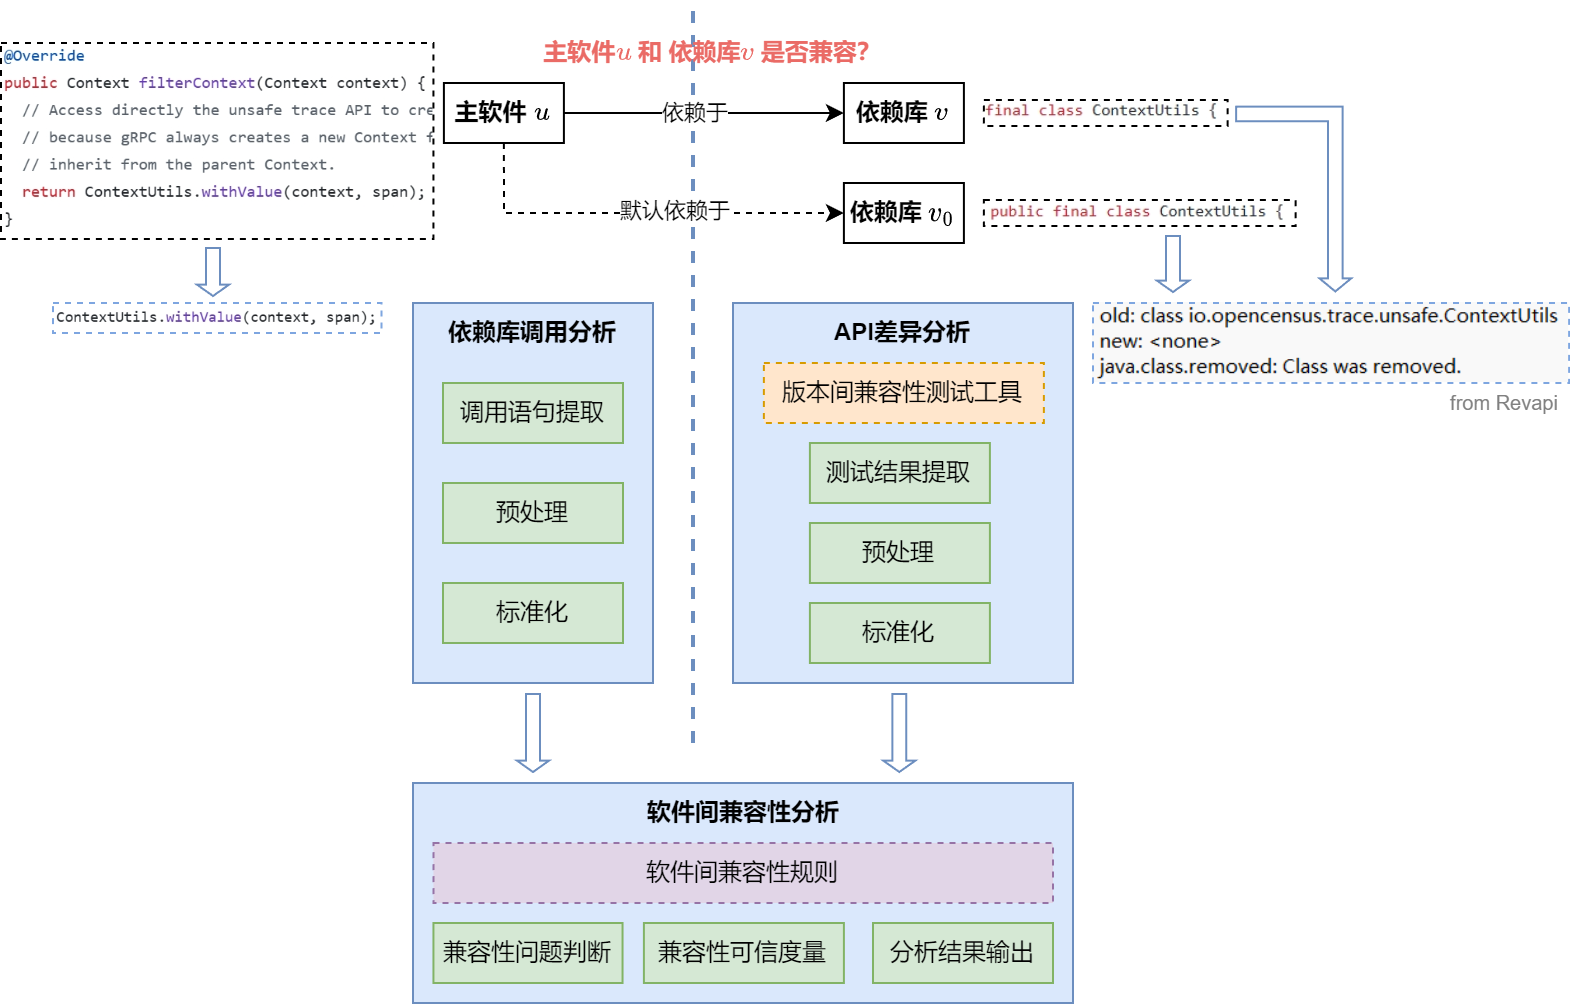
\includegraphics[width=0.9\textwidth]{img/1.png}
	\caption{软件间兼容性测试框架}
\end{figure}

\begin{enumerate}
	\item
	\textbf{依赖库调用分析:}
	
	分析主软件当前版本的源代码,从中提取主软件对直接依赖软件中API调用语句,从而知道有哪些API(类/接口/方法/…)被以何种形式调用(类继承/方法调用/方法重载…)。
	
	\item
	\textbf{API差异分析:}
	
	分析直接依赖软件的当前版本和默认版本中API存在的差异,即API相对于默认版本存在哪些变动(类被移除/方法参数数量变动/方法返回值类型变动…)。该分析可以借助已有的开源版本间兼容性测试工具进行。
	
	\item 
	\textbf{软件间兼容性分析:}
	
	针对从主软件源代码中的提取的API调用语句和直接依赖软件中的API差异,我们要分析这些API差异对API调用造成的影响,因为主软件通常只会调用直接依赖软件提供的部分API。
	
	我们基于预先设定的软件间兼容性规则,来判断是否会存在兼容性问题,以及兼容性问题的严重程度。
\end{enumerate}

值得一提的是,类继承经常引发兼容性问题。当直接依赖软件的某个抽象类中添加了新的抽象方法时,只有主软件继承了该类才会出现兼容性问题,如下图所示:

\begin{figure}[H]
	\centering
	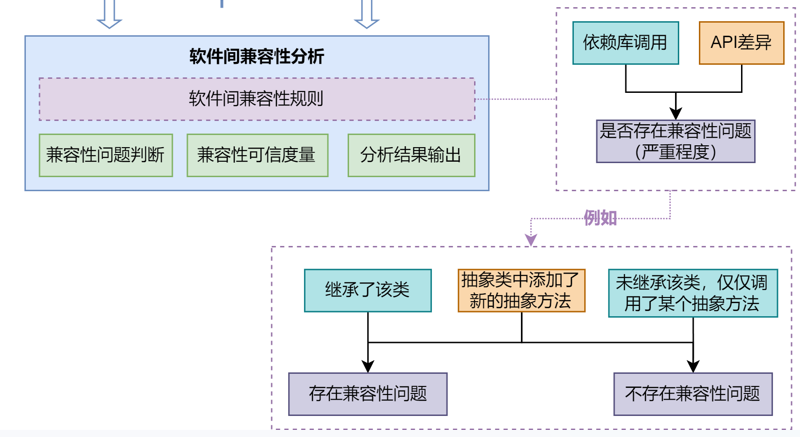
\includegraphics[width=0.9\textwidth]{img/2.png}
	\caption{类继承引发的兼容性问题}
\end{figure}

\subsubsection{Java-Compatibility——面向Java的工具平台框架}

Java-Compatibility工具平台框架是专门设计用于检测和度量Java主软件与其直接依赖的开源软件之间的兼容性的。该框架基于前述软件间兼容性测试框架构建,它整合了静态分析与API差异分析技术,以确保能够准确地评估主软件在引入或升级其依赖项时可能遇到的兼容性问题。以下是Java-Compatibility工具的主要组成部分及其实现细节:

\begin{enumerate}
	\item 
	\textbf{依赖库调用分析}
	
	在这个阶段,Java-Compatibility使用JavaParser框架来解析主软件项目的源代码。通过静态分析,它可以识别出哪些API(类、接口、方法等)被主软件所调用,并提取这些API调用语句。这一步骤至关重要,因为它确定了哪些API变动可能会对主软件产生影响。
	
	\begin{figure}[H]
		\centering
		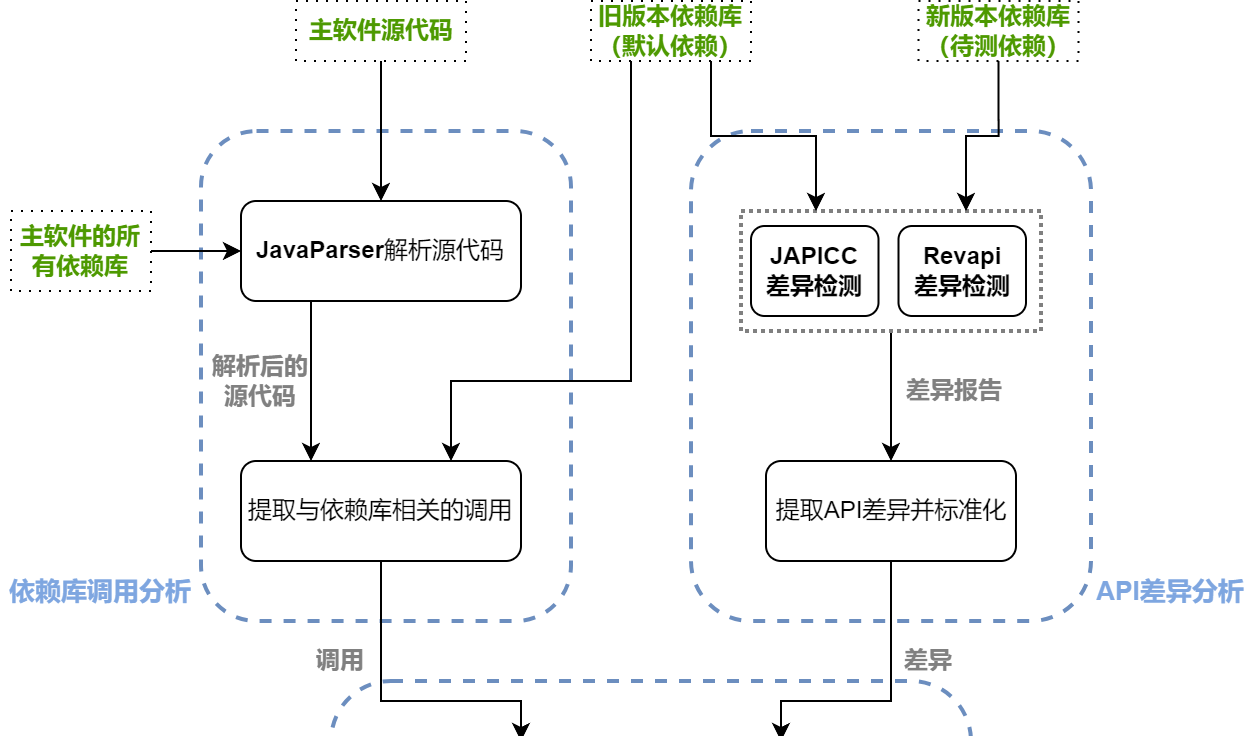
\includegraphics[width=0.7\textwidth]{img/3.png}
		\caption{依赖库调用分析、API差异分析}
	\end{figure}
	
	\item 
	\textbf{API差异分析}
	
	接着,Java-Compatibility会利用JAPICC和Revapi工具来检测直接依赖软件当前版本与默认版本间的API差异。这两个工具可以生成详细的差异报告,指出API签名上的任何变化,如类或方法的添加、移除或修改。此外,Java-Compatibility还会读取并处理这些差异报告,将它们标准化以便后续分析。
	
	\item
	\textbf{软件间兼容性分析}
	
	最后,在拥有主软件的API调用信息以及直接依赖软件的API差异之后,Java-Compatibility会对两者进行综合分析。它基于预先设定的一套软件间兼容性规则,判断API变动是否会导致实际调用中的兼容性问题,并评估这些问题的严重程度。例如,如果一个抽象类中新增了一个抽象方法,并且主软件继承了这个类,则认为存在严重的兼容性问题。
	
	\begin{figure}[H]
		\centering
		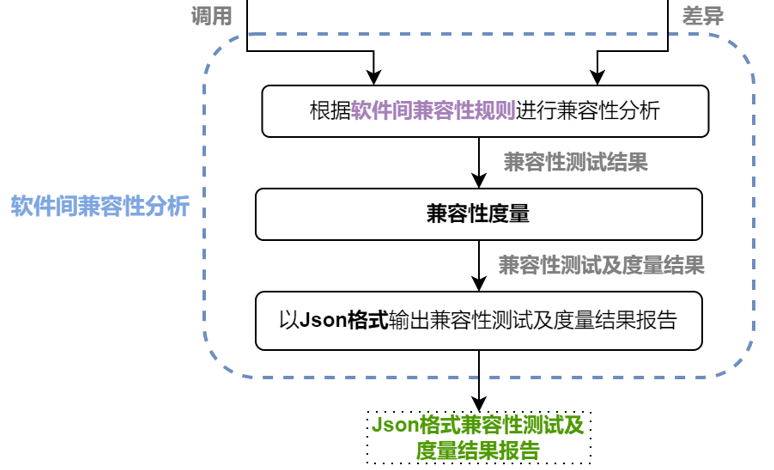
\includegraphics[width=0.5\textwidth]{img/4.png}
		\caption{软件间兼容性分析}
	\end{figure}
\end{enumerate}

Java-Compatibility还实现了共42条针对Java语言的软件间兼容性规则。这些规则是在考虑API差异的基础上制定的,并结合具体的API调用情况。当一个API调用受到多个API差异的影响时,受到影响的严重程度总是取较高的值(即优先级为 High > Medium > Low > No)。下面是一些例子:

\begin{center}
	\begin{tabular}{|c|c|c|c|}
		\hline
		\textbf{API差异} & \textbf{API差异描述} & \textbf{API调用} & \textbf{严重程度等级} \\
		\hline
		Class\_Or\_Interface\_Removed & 移除类/接口 & 调用了该类/接口 & High \\
		\hline
		Method\_Return\_Type\_Changed & 方法返回值类型变动 & 该方法被调用 & Medium \\
		\hline
	\end{tabular}
\end{center}

完成上述步骤后,Java-Compatibility会计算最终的兼容性测试结果,并输出一份JSON格式的结果报告。这份报告不仅包含了检测到的所有兼容性问题及其严重程度,还包括了根据玻尔兹曼熵公式计算得出的软件间兼容性可信度量值T。此值反映了两个软件之间兼容性的可靠程度,范围从1到10不等,数值越大表示兼容性越好。同时,还提供了基于不同严重程度兼容性问题密度的等级划分,帮助用户更直观地理解兼容性状况。

\subsubsection{Cpp-Compatibility——面向C++的工具平台框架}

Cpp-Compatibility工具平台框架是专门为检测和度量C++主软件与其直接依赖的开源软件之间的兼容性而设计的。该框架同样基于前述软件间兼容性测试框架构建,整合了静态分析与API差异分析技术,确保能够准确评估主软件在引入或升级其依赖项时可能遇到的兼容性问题。以下是Cpp-Compatibility工具的主要组成部分及其实现细节:

\begin{enumerate}
	\item 
	\textbf{依赖库调用分析}
	
	在这个阶段,Cpp-Compatibility将主软件源代码与其所有依赖库一同编译(在Linux环境下),并保留调试信息以生成动态链接库(.so)。通过使用pyelftools库读取和分析这些动态链接库中的调试信息,可以提取出主软件对依赖库的API调用情况。这一步骤对于确定哪些API变动可能影响到主软件至关重要。
	
	\begin{figure}[H]
		\centering
		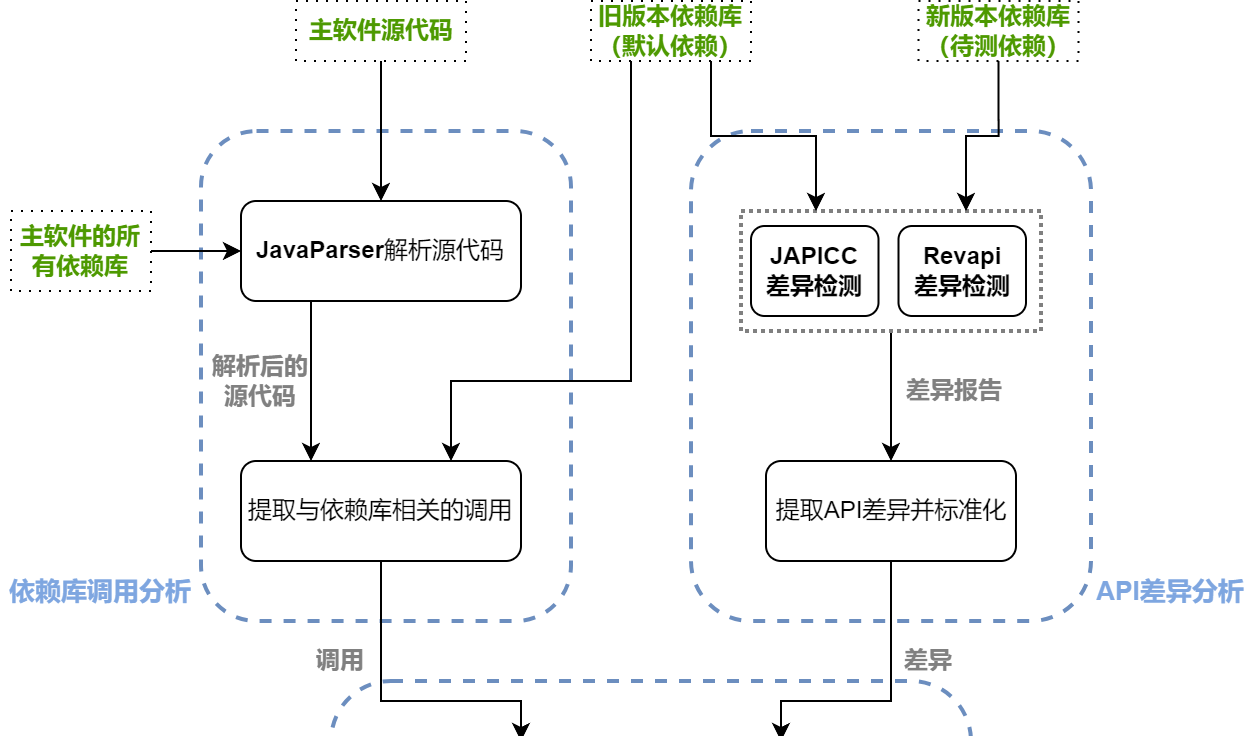
\includegraphics[width=0.7\textwidth]{img/3.png}
		\caption{依赖库调用分析、API差异分析}
	\end{figure}
	
	\item 
	\textbf{API差异分析}
	
	接着,Cpp-Compatibility会利用ABICC工具来检测直接依赖软件当前版本与默认版本间的API差异。ABICC工具能够生成详细的差异报告,指出API签名上的任何变化,如函数、数据类型等的添加、移除或修改。此外,Cpp-Compatibility还会读取并处理这些差异报告,将它们标准化以便后续分析。
	
	\item
	\textbf{软件间兼容性分析}
	
	最后,在拥有主软件的API调用信息以及直接依赖软件的API差异之后,Cpp-Compatibility会对两者进行综合分析。它基于预先设定的一套C/C++软件间兼容性规则,判断API变动是否会导致实际调用中的兼容性问题,并评估这些问题的严重程度。例如,如果一个类中新增了一个纯虚方法,并且主软件继承了这个类,则认为存在严重的兼容性问题。
	
	\begin{figure}[H]
		\centering
		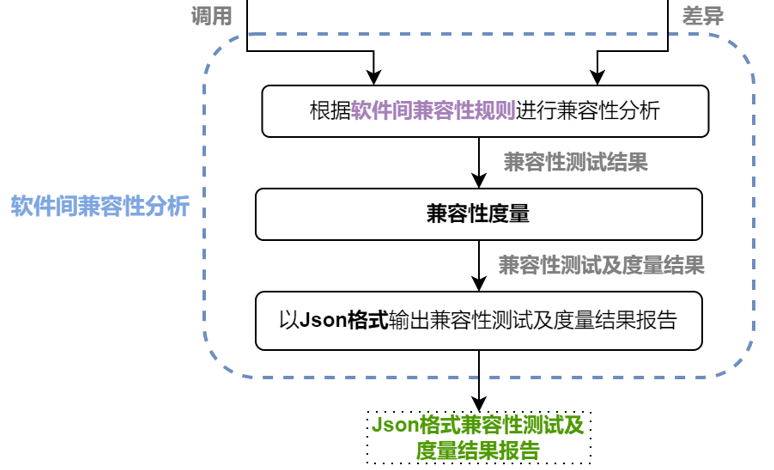
\includegraphics[width=0.5\textwidth]{img/4.png}
		\caption{软件间兼容性分析}
	\end{figure}
\end{enumerate}

Cpp-Compatibility还实现了共66条针对C/C++语言的软件间兼容性规则。这些规则是在考虑API差异的基础上制定的,并结合具体的API调用情况。当一个API调用受到多个API差异的影响时,受到影响的严重程度总是取较高的值(即优先级为 High > Medium > Low > No)。下面是一些例子:

\begin{center}
	\begin{tabular}{|c|c|c|c|c|}
		\hline
		\textbf{API差异} & \textbf{API差异描述} & \textbf{语言限定} & \textbf{API调用} & \textbf{严重程度等级} \\
		\hline
		Removed\_Field & 数据类型中删除字段 & C/C++ & 该字段被调用 & High \\
		\hline
		Added\_Pure\_Virtual\_Method & 类新增纯虚方法 & C++ & 该类被实例化 & High \\
		\hline
		Field\_Pointer\_Level\_Changed & 字段指针等级改变 & C/C++ & 该字段被访问 & Medium \\
		\hline
		Changed\_Constant & 常数值发生改变 & C/C++ & 该常数被引用 & Low \\
		\hline
	\end{tabular}
\end{center}

完成上述步骤后,Cpp-Compatibility会计算最终的兼容性测试结果,并输出一份JSON格式的结果报告。这份报告不仅包含了检测到的所有兼容性问题及其严重程度,还包括了根据玻尔兹曼熵公式计算得出的软件间兼容性可信度量值T。此值反映了两个软件之间兼容性的可靠程度,范围从1到10不等,数值越大表示兼容性越好。同时,还提供了基于不同严重程度兼容性问题密度的等级划分,帮助用户更直观地理解兼容性状况。

此外,Cpp-Compatibility的设计也充分考虑了C++特有的特性,比如虚函数表、名称修饰(name mangling)等,以确保对C++项目的兼容性分析更加精准和全面。具体来说:

\begin{itemize}
	\item \textbf{虚函数表(Vtable)}:C++支持多态性,其中虚函数表用于实现运行时的多态调用。Cpp-Compatibility能够识别虚函数的变化,包括虚函数的添加、删除或重载,这对于保证子类正确覆盖父类的方法非常重要。
	\item \textbf{名称修饰(Name Mangling)}:C++编译器为了区分不同作用域内的同名函数,会在编译过程中对函数名进行修饰。Cpp-Compatibility能够解析这种修饰后的符号,从而准确跟踪API签名的变化,即使原始函数名保持不变。
	\item \textbf{模板(Templates)}:C++中的模板允许创建泛型类和函数。Cpp-Compatibility特别关注模板定义和实例化的变化,因为这些变化可能会导致编译错误或者行为的不一致。
	\item \textbf{异常规范(Exception Specifications)}:C++允许函数声明抛出特定类型的异常。Cpp-Compatibility会检查异常规格的变化,因为这些变化可能影响到程序的异常处理逻辑。
	\item \textbf{内联函数(Inline Functions)}:虽然内联函数主要是一个优化选项,但它们也可能影响二进制兼容性。Cpp-Compatibility会注意内联函数定义的变化,尤其是当这些变化可能导致不同的行为时。
	\item \textbf{宏定义(Macros)}:预处理器宏定义在C++中广泛使用。Cpp-Compatibility会留意宏定义的变化,因为它们可以在编译时改变代码的行为,进而影响到依赖库的兼容性。
\end{itemize}

总而言之,Cpp-Compatibility确保了对C++项目兼容性分析的深度和广度,使得开发者能够在引入新的依赖版本时更有信心地评估潜在的风险。

\end{document}